\section{Análise preliminar dos dados}

Os dados utilizados neste trabalho consistem nas sessões de gravação no
Indaband, no período compreendido entre 01 de janeiro de 2023 até 19 de dezembro
de 2023.

% Metric                         Value
% ---------------------------  -------
% Sessions created               93314
% Sessions published             18845
% Users who added tracks         11968
% Users with published tracks     3630
% Tracks added                  457224
% Fork tracks                   349060
% Tracks published              134004

\begin{table}[H]
  \centering
  \begin{tabular}{|l|l|}
    \hline
    \textbf{Período} & 01/01/2023 a 19/12/2023 \\ \hline
    Sessões criadas & 93.314 \\ \hline
    Sessões publicadas & 18.845 \\ \hline
    Usuários que adicionaram faixas & 11.968 \\ \hline
    Usuários com faixas publicadas & 3.630 \\ \hline
    Faixas adicionadas & 457.224 \\ \hline
    Faixas \textit{forkadas} & 349.060 \\ \hline
    Faixas publicadas & 134.004 \\ \hline
  \end{tabular}
  \caption{Quantidade de sessões, faixas e usuários no período de 01/01/2023 a 19/12/2023.}
  \label{tab_sessoes}
\end{table}

Verifica-se na tabela \ref{tab_sessoes} uma grande quantidade de faixas criadas,
\textit{forkadas} e publicadas na plataforma. Essas faixas são criadas por um
número pequeno de usuários. Por sua vez, na tabela \ref{tab_convites}, a
quantidade de convites enviados e aceitos é ainda menor em relação ao número de
usuários ativos no período.

\begin{table}[htbp]
  \centering
  \begin{tabular}{|l|l|}
    \hline
    \textbf{Período} & 01/01/2023 a 19/12/2023 \\ \hline
    Sessões criadas & 93.315 \\ \hline
    Sessões com convites & 3.984 \\ \hline
    Sessões com participantes & 1.388 \\ \hline
    Convites & 4.619 \\ \hline
    Convites aceitos & 2.799 \\ \hline
    Usuários que convidaram & 592 \\ \hline
    Usuários convidados & 934 \\ \hline
    Usuários que aceitaram convites & 652 \\ \hline
  \end{tabular}
  \caption{Informações sobre convites no período de 01/01/2023 a 19/12/2023.}
  \label{tab_convites}
\end{table}

Em razão desses dois aspectos, o sistema de recomendação \textit{session-based}
proposto prevê qual o próximo usuário cuja faixa será incluída na sessão, dados
os demais usuários com faixas inclusas e do histórico de sessões dos usuários
envolvidos. Por mais que essa abordagem não utilize os convites, ela é capaz de
recomendar usuários que ainda não tenham contribuído para a sessão e que
potencialmente possam contribuir.

Dessa forma, os itens das sessões serão os próprios usuários, e não as faixas,
evitando que o sistema recomende um usuário que já tenha uma faixa incluída na
sessão. Além disso, seguindo a abordagem \textit{session-aware}, o criador de
cada sessão será considerado como o usuário ativo. Isso permite que o sistema
modele as preferências individuais de usuários ao criarem sessões.

\section{\textit{session-rec}} A biblioteca \textit{session-rec} foi
desenvolvida para facilitar experimentos comparando recomendadores
\textit{session-based} em Python. A biblioteca contém as implementações dos
modelos previamente citados no presente trabalho. Um novo modelo pode ser
implementado seguindo o polimofismo das demais implementações.

Cada experimento é declarado em um arquivo .yml, contendo as informações dos
dados a serem utilizados, dos modelos a serem avaliados e de seus hiperparâmetros.

A biblioteca contém um script de pré--processamento, responsável por separar os
dados em conjuntos de treinamento, validação e teste, filtrando os dados de
acordo com o suporte mínimo dos itens e o número mínimo de usuários por sessão,
à escolha do usuário. Em geral, os conjuntos de testes nos comparativos
publicados utilizando a ferramenta é limitado a itens nos dias mais recentes, da
ordem de 1 a 7 dias.

A divisão dos dados pode ser feita de duas formas: \textit{single split} e
\textit{window}. A primeira forma divide o conjunto de dados em um único
conjunto de teste e treinamento. A segunda forma divide a base de dados em
múltiplos conjuntos de acordo com uma janela de tempo especificada. Dessa forma, os
últimos dias de cada conjunto são reservados para teste, enquanto que os dias
anteriores da mesma janela são utilizados para o treinamento.

 Para cada experimento, há dois métodos de avaliação disponíveis: no primeiro,
 avalia-se a capacidade de prever o próximo item imediato da sessão. No segundo,
 avalia-se a capacidade de prever todos os itens subsequentes da sessão.

\section{\textit{Experimentos}} 



% \begin{table}[htbp]
%   \centering
%   \begin{tabular}{|l|l|l|l|}
%     \hline
%       & Eventos & Sessões & Itens \\ \hline
%      \textit{Dataset} completo & 154.121 & 77.055 & 20.840 \\ \hline
%       \textit{Dataset} filtrado & 105.955 & 31.103 & 2.579 \\ \hline
%       Conjunto completo de treinamento & 99.714 & 29.328 & 2.452 \\ \hline
%       conjunto de teste & 5.516 & 1.530 & 477 \\ \hline
%       Conjunto de treinamento & 93.679 & 27.605 & 2.320 \\ \hline
%       Conjunto de validação & 5.291 & 1.467 & 475 \\ \hline
%       Conjunto de otimização & 304 & 100 & 111 \\ \hline
%   \end{tabular}
%   \caption{Informações sobre o \textit{dataset} utilizado na abordagem \textit{single}.}
%   \label{tab_dataset}
% \end{table}

\subsection{Abordagem \textit{single-split}}

\citet{HidasiKBT15} utiliza a abordagem \textit{single-split} para comparar a
avaliação dos modelos, de forma que o conjunto de treinamento é composto pelos
últimos seis meses, enquanto que o conjunto de teste é composto pelo último dia
do conjunto completo \cite{ludewig_2018}. Essa é a abordagem mais próxima de um
modelo em produção.

O \textit{dataset} é dividido segundo a abordagem \textit{single split}, em um
único conjunto de treinamento e teste, tal como na tabela
\ref{tab:split_data}. Nesses experimentos, os modelos de base de comparação
desconsideram o usuário dono da sessão. Dessa forma, não há modelos
\textit{session-aware}.

Apenas sessões com um mínimo de dois usuários estão presentes, como ilustrado na
figura \ref{fig:next-item-single}. Similarmente, o suporte mínimo dos itens é
igual a 2. Dessa forma, há apenas usuários que constam em pelo menos duas
sessões publicadas.

Na abordagem apresentada, apenas a primeira interação de cada usuário na
sessão consta na base, de forma que nenhum usuário apareça mais de uma vez na
mesma sessão.
  \begin{table}[htbp]
    \centering
    \begin{tabular}{|l|l|l|l|l|l|l|}
      \hline
      Conjunto & Eventos & Sessões & Itens & $\Delta$ & $\sigma$ & Janela de tempo \\ \hline 
         Treinamento & 90.801 & 26.649 & 1.702 & 3,3 & 2,0 & 01/01/2023 a 03/12/2023 \\ \hline
        Teste & 11.265 & 3.106 & 589 & 3,6 & 2,0 & 02/08/2023 a 18/12/2023 \\ \hline
    \end{tabular}
    \caption{Informações sobre o \textit{dataset} utilizado na abordagem
    \textit{single}. $\Delta$ e $\sigma$ são a média e o desvio padrão da quantidade de
    usuários por sessão.}
    \label{tab:split_data}
  \end{table}

  \begin{figure}[ht]
    \centering
    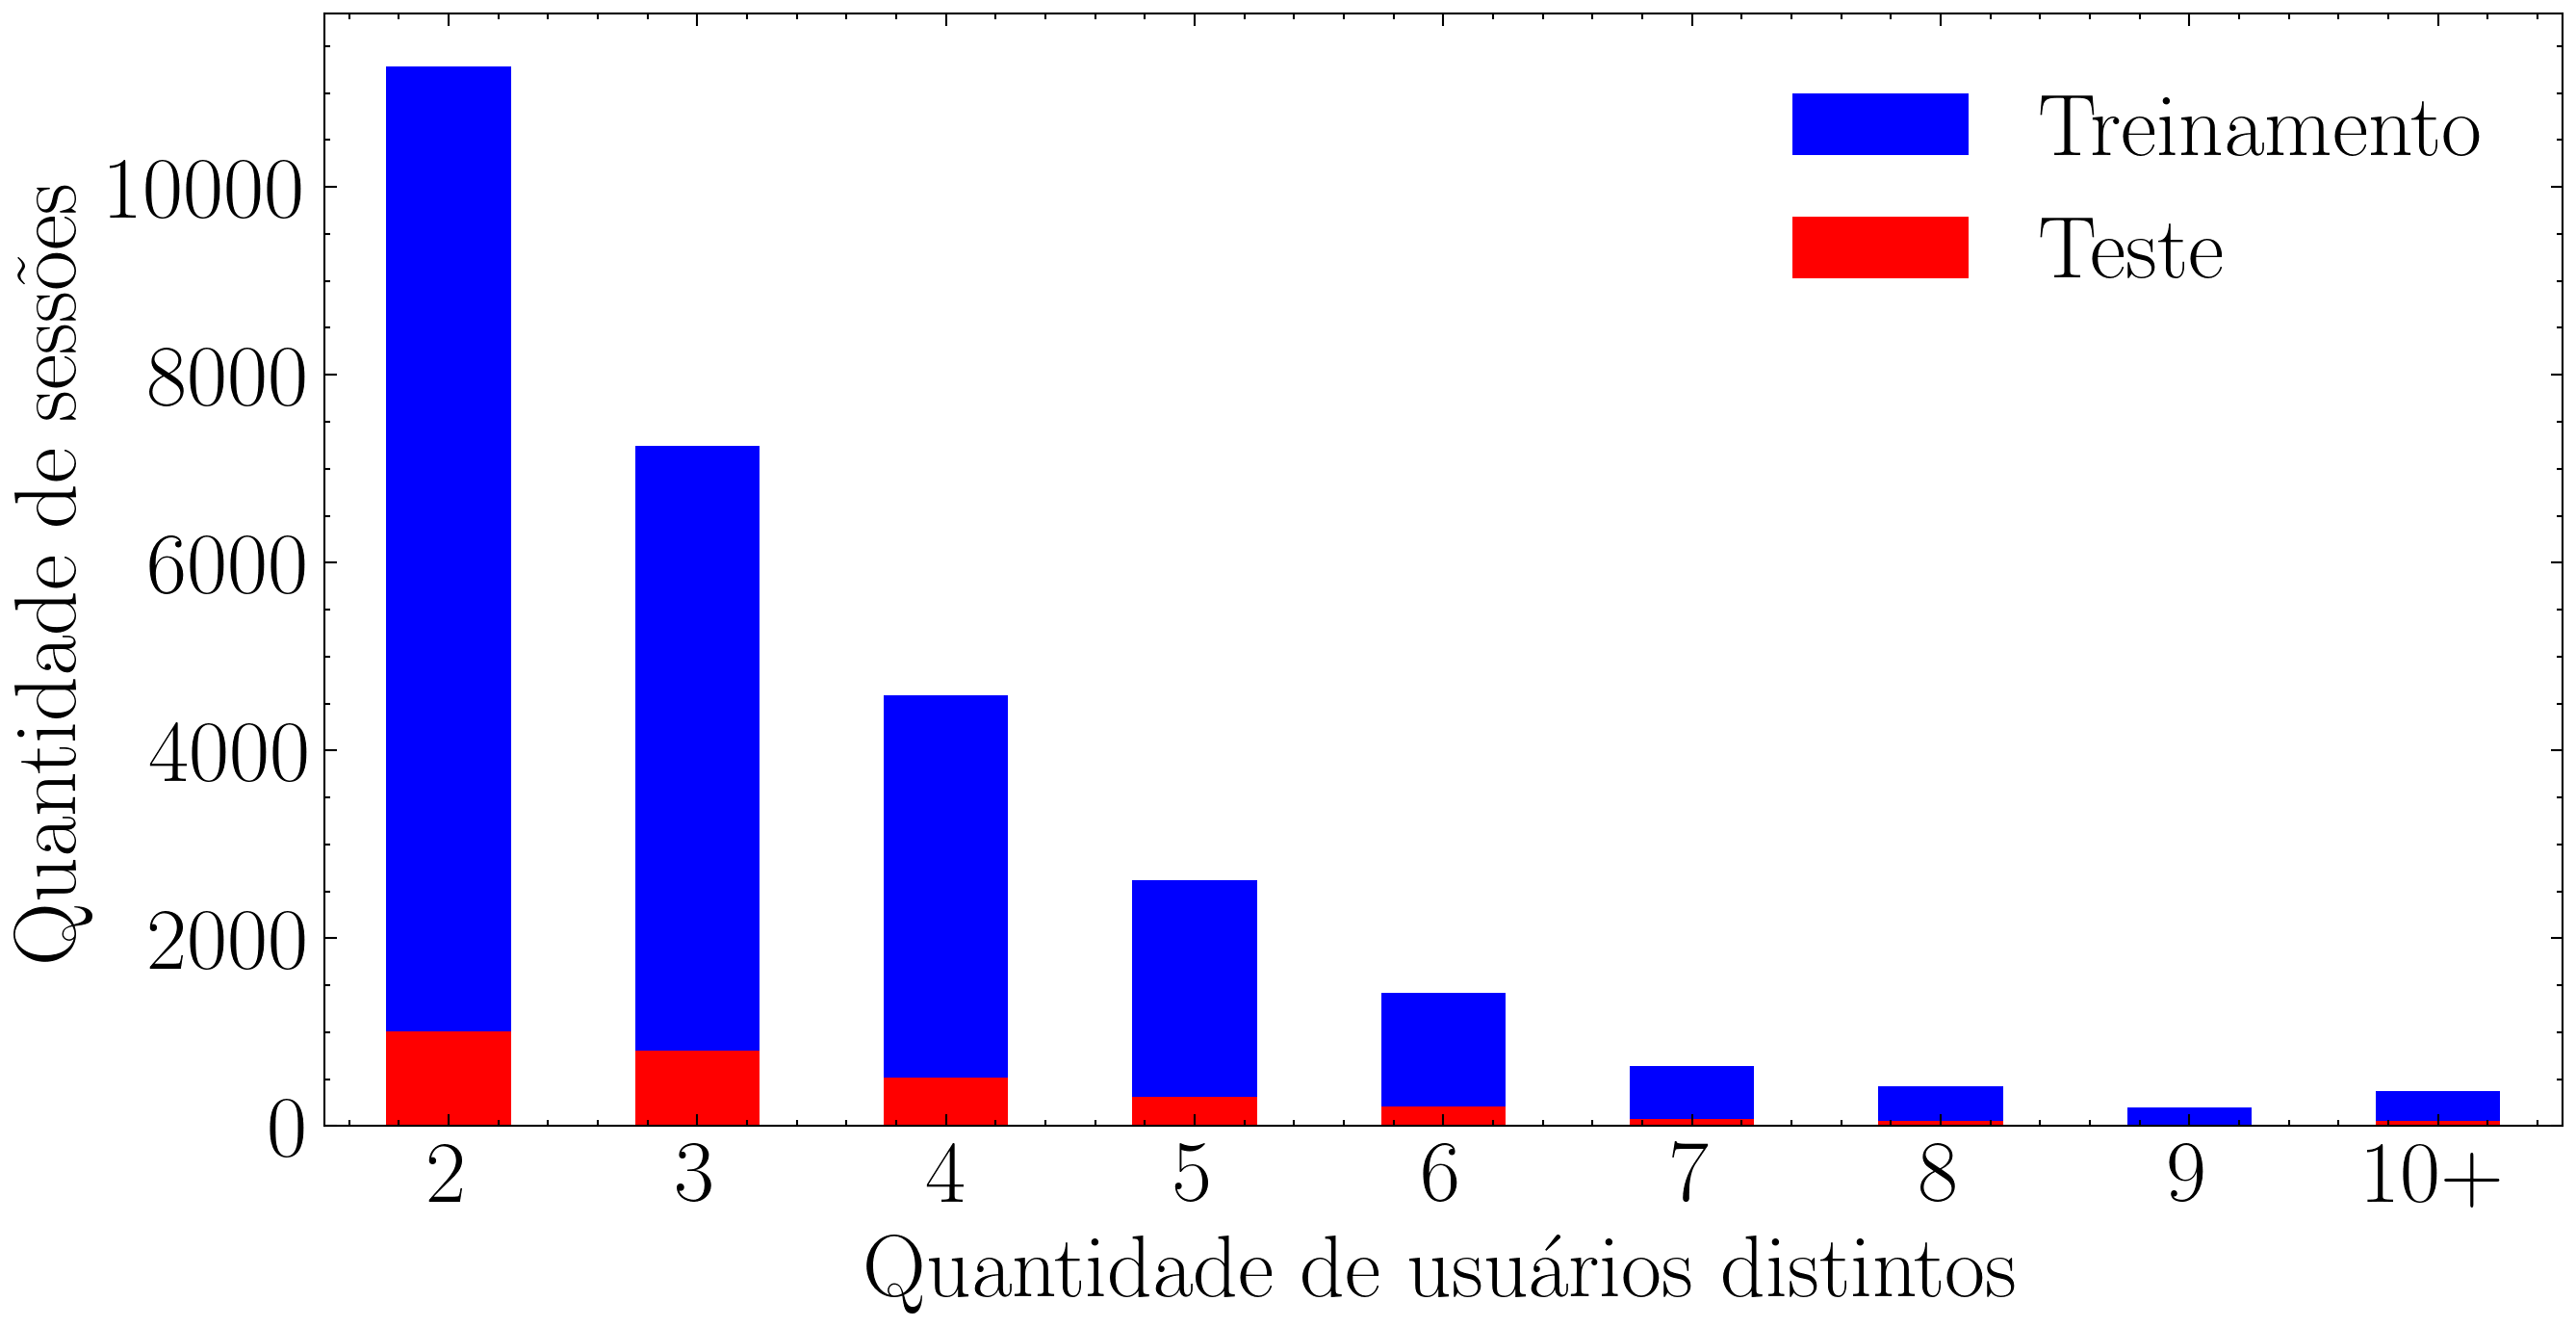
\includegraphics[width=1\textwidth]{chapters/chap04/images/histograma.png}
    \caption{Distribuição da quantidade de usuários por sessão na abordagem
    \textit{single}. A distribuição de treinamento está empilhada acima da
    distribuição de teste.}
    \label{fig:next-item-single}
  \end{figure}
 

  \subsubsection{Modelos não-personalizados}

  Pop é o modelo de popularidade, com pontuações proporcionais ao suporte dos
  itens, limitado aos 100 itens mais populares. Random é o modelo aleatório,
  retornando uma pontuação aleatória para cada item. SPop é o modelo de
  popularidade de sessão, em que as pontuações são proporcionais à maior
  frequência dos itens em cada sessão, também limitado aos 100 itens mais
  populares. Finalmente, RPop é o modelo de popularidade para sessões recentes,
  em que apenas itens do último dia são considerados por padrão. Foi utilizada a
  avaliação sobre o próximo item da sessão.
\begin{table}[htbp]
  \centering
  \begin{tabular}
    {|l|l|l|l|l|l|l|l|}
    \hline
    Modelo & HR@5 & HR@10 & MRR@5 & MRR@10 & NDCG@10 & Cov@10 & Pop@10 \\ \hline
    Pop & 0,132 & 0,268 & 0,092 & 0,110 & 0,155 & 0,006 & 0,531 \\ \hline
    Random & 0,003 & 0,006 & 0,001 & 0,002 & 0,003 & \textbf{1,000} & \textbf{0,013} \\ \hline
    RPop & \textbf{0,204} & \textbf{0,294} & \textbf{0,125} & \textbf{0,137} & \textbf{0,204} & 0,010 & 0,321 \\ \hline
    SPop & 0,109 & 0,221 & 0,045 & 0,058 & 0,114 & 0,301 & 0,473 \\ \hline
  \end{tabular}
  \caption{Resultados obtidos com os modelos de base de comparação não-personalizados, avaliando a predição do próximo item da sessão.}
\end{table}

De forma esperada, o modelo Random maximiza a cobertura, minimizando o índice de
popularidade. O modelo de popularidade para sessões recentes (RPop) apresenta
resultados superiores aos demais modelos de popularidade.


\subsubsection{Modelos por mineração de padrões e vizinhança}

\begin{table}[htbp]
  \centering
  \begin{tabular}{|l|l|l|l|l|l|l|l|}
    \hline
    Modelo & HR@5 & HR@10 & MRR@5 & MRR@10 & Cov@10 & Pop@10 & $\Delta t_{treino} [s]$ \\
    \hline
    Markov  & 0,465 & 0,583 & \textbf{0,292} & 0,308 & 0,488 & 0,247 & 0.1 \\
    \hline
    AR & 0,403 & 0,531 & 0,238 & 0,255 & 0,488 & 0,284 & 0.1 \\
    \hline
    $\text{SR}_{1}$ & 0,461 & 0,583 & 0,291 & 0,308 & 0,492 & 0,272 & 0.1 \\
    \hline
    $\text{SR}_{2}$ & \textbf{0,468} & 0,593 & \textbf{0,292} & \textbf{0,310} & 0,507 & 0,260 & 0.1 \\
    \hline
    $\text{skNN}_{1}$ & 0,406 & 0,564 & 0,151 & 0,172 & \textbf{0,636} & \textbf{0,187} & 0.1 \\
    \hline
    $\text{skNN}_{2}$ & 0,444 & \textbf{0,604} & 0,157 & 0,179 & 0,603 & 0,217 & 0.1 \\
    \hline
    $\text{vsKNN}_{1}$ & 0,365 & 0,527 & 0,136 & 0,158 & 0,312 & 0,222 & 0.1 \\
    \hline
    $stan_{1}$ & 0,403 & 0,570 & 0,147 & 0,170 & 0,516 & 0,271 & 0.1 \\
    \hline
    $stan_{2}$ & 0,366 & 0,551 & 0,126 & 0,151 & 0,562 & 0,196 & 0.1 \\
    \hline
    $vstan_{1}$ & 0,419 & 0,573 & 0,161 & 0,182 & 0,553 & 0,230 & 0.1 \\
    \hline
    $vstan_{2}$ & 0,412 & 0,582 & 0,148 & 0,171 & 0,571 & 0,236 & 0.1 \\
    \hline
  \end{tabular}
  \caption{Resultado para os modelos de base de comparação, avaliando o próximo item da sessão.
  Os hiperparâmetros utilizados para cada modelo estão descritos no apêndice.}
  %  $\text{SR}_{1}$
  % e $\text{SR}_{2}$ são os modelos de regras de sequência com 6 e 11 passos, com peso inverso e quadrático.
  % $\text{skNN}_{1}$ e $\text{skNN}_{2}$ são os modelos de kNN com 50 e 100 vizinhos, ambos com função de similaridade cosseno.
  % $\text{vsKNN}_{1}$ e $\text{vsKNN}_{2}$ são os modelos de kNN com 1500 e 50 vizinhos, com amostragem de 10.000 e 2.500, respectivamente, ambos com função de similaridade cosseno.
  % vstan-k=1000-sample_size=5000-similarity=cosine-lambda_spw=10-lambda_snh=40-lambda_inh=5-lambda_ipw=1e-05-lambda_idf=False
  % vstan-k=2000-sample_size=1000-similarity=vec-lambda_spw=10-lambda_snh=100-lambda_inh=0.625-lambda_ipw=0.125-lambda_idf=False
  % $stan_{1}$ e $stan_{2}$ são os modelos de kNN com 1000 e 2000 vizinhos, com
  % amostragem de 5000 e 1000, respectivamente, com função de similaridade
  % cosseno e vetorial,   
  \label{tab_baseline}  
\end{table}

Em seguida, é realizada a avaliação para predição do próximo item em modelos de
mineração de padrões: regras de associação, cadeias de Markov, regras de
sequência. Também é realizada para métodos de vizinhança: kNN, vskNN, stan e
vstan. Os modelos SR, skNN e vsKNN são avaliados com hiperparâmetros distintos,
obtidos a partir de uma otimização do MRR@10, cujas métricas constam na tabela
\ref{tab_baseline}. Os melhores resultados foram obtidos com os modelos
$\text{SR}_{2}$ e $\text{skNN}_{2}$, ambos otimizados.






\subsubsection{métodos baseados em fatoração}
Em seguida, são avaliados os modelos baseados em fatoração: FPMC, FISM, Fossil
e BPRMF.

\begin{table}[htbp]
  \centering
  \begin{tabular}{|l|l|l|l|l|l|l|l|}
    \hline
    Modelo & HR@5 & HR@10 & MRR@5 & MRR@10 & Cov@10 & Pop@10 & $\Delta t_{treino} [s]$ \\
    \hline
    FPMC & \textbf{0,289} & \textbf{0,421} & 0,122 & 0,140 & 0,840 & \textbf{0,226} & 921,7 \\
    \hline
    FISM & 0,280 & 0,414 & \textbf{0,126} & \textbf{0,144} & 0,824 & 0,264 & 918,7 \\
    \hline
    Fossil & 0,243 & 0,399 & 0,100 & 0,121 & \textbf{0,848} & 0,253 & 917,7 \\
    \hline
    BPRMF & 0,253 & 0,397 & 0,107 & 0,125 & 0,834 & 0,233 & 918,3 \\
    \hline
  \end{tabular}
  \caption{Resultado para os modelos baseados em fatoração, avaliando o próximo item da sessão.}
  \label{tab_fatoracao}
\end{table}

\subsubsection{Modelos baseados em redes neurais}
Em seguida, são avaliados os modelos baseados em redes neurais: GRU4Rec, NARM,
STAMP e Caser.

\subsection{Comparativo entre abordagem \textit{windowed} e \textit{single-split}}

Algumas das limitações da abordagem \textit{single-split} envolvem a maior
suscetibilidade a efeitos aleatórios e a particularidades dos dados. Uma
alternativa é a abordagem \textit{windowed}, que minimiza os riscos de os
resultados serem influenciados por uma única configuração de treino e teste. A
abordagem \textit{windowed} equivale a uma validação cruzada, com a limitação de
que os dados são ordenados cronologicamente. \citet{ludewig_2018} divide os
dados em cinco janelas de um mês, em que o último dia de cada janela é reservado
para teste. O resultado final para as métricas é a média aritmética dos
métricas obtidas em cada janela.

A seguir, são apresentados os resultados obtidos com a abordagem
\textit{windowed}. Uma janela deslizante é aplicada por todo o período,
separando em cinco pares distintos de treinamento e teste, descritos na tabela
\ref{tab:windowed_data}. Nota-se o aumento gradual da quantidade de eventos,
sessões e itens ao longo do tempo.

\begin{table}[htbp]
  \centering
  \begin{tabular}{|c|c|c|c|c|c|}
    \hline
    Conjunto & Índice & Eventos & Sessões & Itens & Data\\
    \hline
    Treinamento & 1 & 3190 & 1098 & 145 & 08/01/2023 a 09/03/2023\\
    \hline
    Teste & 1 & 205 & 72 & 40 & 09/03/2023 a 13/03/2023\\
    \hline
    Treinamento & 2 & 3976 & 1346 & 197 & 14/03/2023 a 13/05/2023\\
    \hline
    Teste & 2 & 244 & 68 & 53 & 13/05/2023 a 17/05/2023\\
    \hline
    Treinamento & 3 & 7407 & 2191 & 301 & 18/05/2023 a 17/07/2023\\
    \hline
    Teste & 3 & 466 & 162 & 100 & 17/07/2023 a 21/07/2023\\
    \hline
    Treinamento & 4 & 21683 & 6267 & 754 & 22/07/2023 a 20/09/2023\\
    \hline
    Teste & 4 & 1779 & 454 & 201 & 20/09/2023 a 24/09/2023\\
    \hline
    Treinamento & 5 & 43993 & 12852 & 1681 & 25/09/2023 a 24/11/2023\\
    \hline
    Teste & 5 & 2978 & 830 & 351 & 24/11/2023 a 28/11/2023\\
    \hline
  \end{tabular}
  \caption{Conjuntos de treino e teste separados em cinco janelas.}
  \label{tab:windowed_data}
\end{table}

Os resultados sob abordagem \textit{windowed} são obtidos a partir da média
aritmética dos resultados obtidos em cada janela.

% "",Metrics,HitRate@5:,HitRate@10:,MRR@5:,MRR@10:,Coverage@10:,Popularity@10:,Saver@10:,Training time:,Unnamed: 11
% 0,pop,0.202483,0.325002,0.113988,0.130352,0.034432,0.492751,1,0.001799,NaN
% 1,random,0.011728,0.031881,0.006648,0.009480,1.000000,0.044801,1,0.000095,NaN
% 2,rpop,0.221616,0.356404,0.115727,0.133340,0.065223,0.355387,1,0.006027,NaN
% 3,spop,0.167503,0.297867,0.071662,0.088933,0.235196,0.455571,1,0.004045,NaN
% 4,fpmc,0.290820,0.437599,0.140368,0.159389,0.613081,0.350379,1,897.077106,NaN
% 5,fism,0.290769,0.443388,0.144321,0.164441,0.625496,0.345538,1,892.356516,NaN
% 6,fossil,0.288414,0.416936,0.146647,0.163657,0.605429,0.342610,1,900.197152,NaN
% 7,bprmf,0.290234,0.421054,0.149111,0.166053,0.624408,0.343189,1,893.929285,NaN
% 8,markov,0.360468,0.477359,0.217812,0.233454,0.437617,0.256820,1,0.046681,NaN
% 9,ar,0.363188,0.475916,0.207177,0.221873,0.454511,0.299607,1,0.116567,NaN
% 10,sr-steps=15-weighting=div,0.378248,0.505640,0.225488,0.241997,0.443499,0.280725,1,0.097471,NaN
% 11,sr-steps=6-weighting=quadratic,0.374524,0.508404,0.224006,0.241340,0.452892,0.272955,1,0.105958,NaN
% 12,sknn-k=50-sample_size=500-similarity=cosine,0.350581,0.526155,0.139853,0.163773,0.533600,0.257608,1,0.078924,NaN
% 13,sknn-k=100-sample_size=2500-similarity=cosine,0.333647,0.507204,0.132399,0.155586,0.491283,0.281977,1,0.058884,NaN
% 14,vsknn-k=1500-sample_size=10000-weighting=quadratic-weighting_score=linear-idf_weighting=10,0.299105,0.458049,0.118672,0.139682,0.511241,0.267182,1,0.079672,NaN
% 15,vsknn-k=50-sample_size=2500-weighting=same-weighting_score=div-idf_weighting=1,0.340011,0.477184,0.131604,0.149647,0.533716,0.232979,1,0.077049,NaN
% 16,stan-k=2000-sample_size=2500-lambda_spw=3.62-lambda_snh=100-lambda_inh=7.24,0.339429,0.493634,0.131960,0.152665,0.462927,0.324394,1,0.058802,NaN
% 17,stan-k=100-sample_size=2500-lambda_spw=1.81-lambda_snh=40-lambda_inh=0.197,0.345886,0.492803,0.128909,0.148756,0.505962,0.261668,1,0.092315,NaN
% 18,vstan-k=1000-sample_size=5000-similarity=cosine-lambda_spw=10-lambda_snh=40-lambda_inh=5-lambda_ipw=1e-05-lambda_idf=False,0.362617,0.505379,0.144631,0.164285,0.486622,0.291301,1,0.061980,NaN
% 19,vstan-k=2000-sample_size=1000-similarity=vec-lambda_spw=10-lambda_snh=100-lambda_inh=0.625-lambda_ipw=0.125-lambda_idf=False,0.358136,0.493258,0.137204,0.155337,0.499507,0.293144,1,0.066452,NaN


\begin{table}
  \centering
  \begin{tabular}{|l|l|l|l|l|l|l|l|}
    \hline
    Modelo & HR@5 & HR@10 & MRR@5 & MRR@10 & Cov@10 & Pop@10 & $\Delta t_{treino} [s]$ \\
    \hline
    Pop & 0,202 & 0,325 & 0,114 & 0,130 & 0,034 & 0,493 & 0,001 \\
    \hline
    Random & 0,012 & 0,032 & 0,007 & 0,009 & 1,000 & 0,045 & 0,001 \\
    \hline
    RPop & 0,222 & 0,356 & 0,116 & 0,133 & 0,065 & 0,355 & 0,006 \\
    \hline
    SPop & 0,168 & 0,298 & 0,072 & 0,089 & 0,235 & 0,456 & 0,004 \\
    \hline
    FPMC & 0,291 & 0,438 & 0,140 & 0,159 & 0,613 & 0,350 & 897 \\
    \hline
    FISM & 0,291 & 0,443 & 0,144 & 0,164 & \textbf{0,625} & 0,346 & 892 \\
    \hline
    Fossil & 0,288 & 0,417 & 0,147 & 0,164 & 0,605 & 0,343 & 900 \\
    \hline
    BPRMF & 0,290 & 0,421 & 0,149 & 0,166 & 0,624 & 0,343 & 893 \\
    \hline
    $smf_{1}$ & \textbf{0,401} & 0,532 & \textbf{0,247} & \textbf{0,264} & 0,492 & 0,281 & 193 \\
    \hline
    $smf_{2}$ & 0,364 & 0,495 & 0,224 & 0,240 & 0,271 & 0,328 & 162 \\
    \hline
    Markov & 0,360 & 0,477 & 0,218 & 0,233 & 0,438 & 0,257 & 0,047 \\
    \hline
    AR & 0,363 & 0,476 & 0,207 & 0,222 & 0,455 & 0,300 & 0,117 \\
    \hline
    $\text{SR}_{1}$ & 0,378 & 0,506 & 0,225 & \textbf{0,242} & 0,443 & 0,281 & 0,097 \\
    \hline
    $\text{SR}_{2}$ & 0,375 & 0,508 & 0,224 & 0,241 & 0,453 & 0,273 & 0,106 \\
    \hline
    $\text{skNN}_{1}$ & 0,351 & \textbf{0,526} & 0,140 & 0,164 & 0,534 & 0,258 & 0,079 \\
    \hline
    $\text{skNN}_{2}$ & 0,334 & 0,507 & 0,132 & 0,156 & 0,491 & 0,282 & 0,059 \\
    \hline
    $\text{vsKNN}_{1}$ & 0,299 & 0,458 & 0,119 & 0,140 & 0,511 & 0,267 & 0,080 \\
    \hline
    $stan_{1}$ & 0,340 & 0,477 & 0,132 & 0,150 & 0,534 & \textbf{0,233} & 0,077 \\
    \hline
    $stan_{2}$ & 0,346 & 0,493 & 0,129 & 0,149 & 0,506 & 0,262 & 0,092 \\
    \hline
  \end{tabular}
  \caption{Resultado dos modelos \textit{session-based}, avaliando o próximo item da sessão. }
\end{table}

\subsection{Abordagem \textit{windowed} \textit{session-aware}}

\begin{table}[htbp]
  \centering
  \begin{tabular}{|c|c|c|c|c|c|c|}
    \hline
    Conjunto & Índice & Eventos & Usuários & Sessões & Itens & Data -- 2023\\
    \hline
    Treino & 1 & 2705 & 76 & 721 & 124 & 01/08 a 13/03\\
    \hline
    Teste & 1 & 245 & 73 & 73 & 75 & 16/03 a 13/03\\
    \hline
    Validação -- Treino & 1 & 2427 & 76 & 645 & 119 & 01/08 a 12/03\\
    \hline
    Validação -- Teste & 1 & 269 & 74 & 74 & 75 & 16/01 a 13/03\\
    \hline
    Treino & 2 & 3463 & 74 & 898 & 160 & 14/03 a 17/05\\
    \hline
    Teste & 2 & 256 & 73 & 73 & 87 & 20/03 a 17/05\\
    \hline
    Validação -- Treino & 2 & 3186 & 74 & 824 & 158 & 14/03 a 17/05\\
    \hline
    Validação -- Teste & 2 & 275 & 74 & 74 & 93 & 20/03 a 17/05\\    
    \hline
    Treino & 3 & 6620 & 109 & 1520 & 270 & 18/05 a 21/06\\
    \hline
    Teste & 3 & 368 & 108 & 108 & 123 & 01/06 a 21/07\\
    \hline
    Validação -- Treino & 3 & 6226 & 109 & 1411 & 265 & 18/05 a 21/07\\
    \hline
    Validação -- Teste & 3 & 386 & 106 & 106 & 130 & 23/05 a 21/07\\
    \hline
    Treino & 4 & 15180 & 308 & 3143 & 581 & 21/07 a 24/09\\
    \hline
    Teste & 4 & 1614 & 305 & 305 & 318 & 23/07 a 24/09\\
    \hline
    Validação -- Treino & 4 & 13483 & 308 & 2835 & 556 & 21/07 a 24/09\\
    \hline
    Validação -- Teste & 4 & 1630 & 298 & 298 & 305 & 22/07 a 24/09\\
    \hline
    Treinamento & 5 & 23244 & 646 & 4369 & 1092 & 24/09 a 28/11\\
    \hline
    Teste & 5 & 3317 & 629 & 629 & 670 & 30/09 a 28/11\\
    \hline
    Validação -- Treino & 5 & 19820 & 646 & 3723 & 1027 & 24/09 a 28/11\\
    \hline
    Validação -- Teste & 5 & 3288 & 625 & 625 & 676 & 26/09 a 28/11\\
    \hline
  \end{tabular}
\end{table}

% \section{Tratamento dos dados}
% Sob a perspectiva comercial, o seguinte indício sustenta que um SBRS pode
% aumentar a taxa de sessões publicadas pelos usuários do Indaband: apenas 1.146
% (7,77\%) das 14.750 sessões criadas em 2023 até 13 de agosto contém no mínimo um
% convite emitido. Afunilando ainda mais, a análise das taxas de publicação indica
% que as sessões com ao menos um convite aceito, que são apenas 349 (2,37\%) das
% 14.750 sessões totais criadas, tem maior taxa de publicação se comparada ao
% conjunto de todas as sessões. Portanto, uma forma simples de aumentar a taxa de
% publicação geral da plataforma é permitir que o conjunto de sessões com
% convidados seja maior, o que pode ser incentivado ao integrar um SBRS ao
% aplicativo.

% Sob a perspectiva de viabilidade técnica, de todas as 14.750 sessões criadas
% em 2023 até 13 de agosto, 6.857 (46,5\%) foram criadas com ao menos dois
% usuários que gravaram as faixas existentes. Isso é possível a partir da
% funcionalidade de \textit{fork}, que permite a cópia de uma sessão publicada
% com suas faixas originais. Basta um novo usuário versionar uma sessão com uma
% única faixa de outro usuário para que exista associações entre esse novo
% usuário e os demais que o segundo usuário já tenha colaborado.

% \vspace{0.2cm}
% \begin{figure}[H]
%       \centering
%       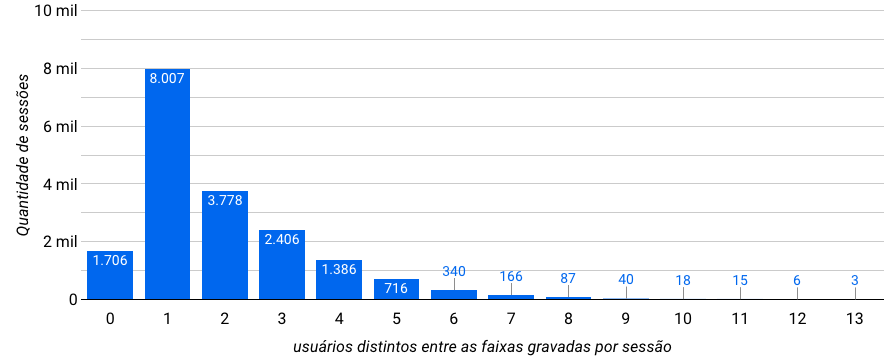
\includegraphics[width=1\textwidth]{chapters/chap01/images/plots/users.png}\vfill
%       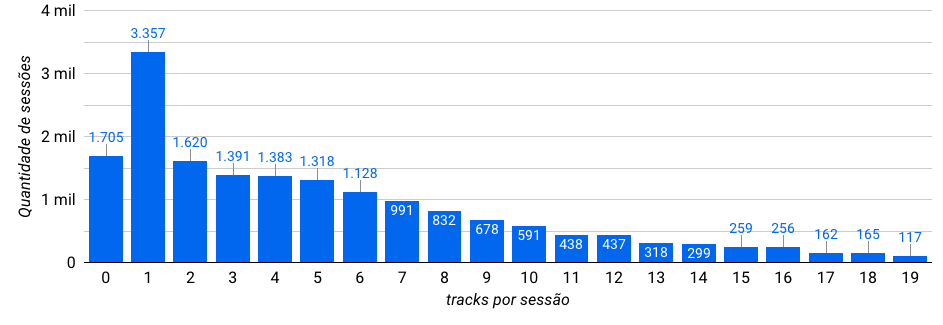
\includegraphics[width=1\textwidth]{chapters/chap01/images/plots/tracks.png}
%       \caption{Dados de sessões em 2023 até o presente momento. A quantidade de \textit{tracks}
%        e usuários por sessão sustenta a viabilidade técnica de um modelo de
%        aprendizado de máquina para a recomendação de convites.}
%       \label{fig:combined}
%   \end{figure}
% \vspace{0.2cm}

% \vspace{0.2cm}
% \begin{figure}[ht]
%     \centering
%     \begin{tikzpicture}
%     \pie[ sum=auto, radius=1.4, color={blue!70, orange!70}, after number=\%,
%       explode={0, 0.1}, text={}, pos={0,-1}, ]{ 41.3/Publicadas, 58.7/Não
%       Publicadas } \node[align=center] at (0,-3) {Total de Sessões: 14.750};
%     \end{tikzpicture}
%     \hspace{1cm} 
%     \begin{tikzpicture}
%     \pie[ sum=auto, radius=0.8, color={blue!70, orange!70}, after number=\%,
%       explode={0, 0.1}, text=legend, pos={0,-1}, ]{ 48.4/Publicadas, 51.6/Não
%       Publicadas } \node[align=center] at (0,-3) {Sessões com 1 convite aceito
%       ou mais: 349};
%     \end{tikzpicture}
%     \caption{Sessões e convites enviados. 01/01/2023 a 13/08/2023. Sessões com convites aceitos têm maior taxa de publicação se comparadas ao conjunto completo.}
%     \end{figure}
%     \vspace{0.2cm}
 
